% Load Configuration
%	Pakete und Konfigurationen
%----------------------------------------------------------------------------------------
%\documentclass[twoside,twocolumn]{article}
\documentclass[oneside,bibliography=totocnumbered,BCOR=5mm]{scrbook}% Voreinstellungen entfernt.

\usepackage[latin1]{inputenc}
\usepackage{amsmath, amsthm, amssymb}
\usepackage[english]{babel} % Language hyphenation and typographical rules
\usepackage{marvosym}
\usepackage{graphicx}
\usepackage{csquotes}
\usepackage[hyphens]{url}
\usepackage[hidelinks]{hyperref}


%----------------------------------------------------------------------------------------
%	BIB.-Datei und Quellenverwaltung
%----------------------------------------------------------------------------------------
\usepackage[backend=biber, style=numeric, sorting=none]{biblatex}
\addbibresource{references/references.bib}
%\usepackage{natbib} % use natbib for references 
%----------------------------------------------------------------------------------------
\usepackage{blindtext} % Package to generate dummy text throughout this template 

\usepackage[sc]{mathpazo} % Use the Palatino font
\usepackage[T1]{fontenc} % Use 8-bit encoding that has 256 glyphs
\linespread{1.05} % Line spacing - Palatino needs more space between lines
\usepackage{microtype} % Slightly tweak font spacing for aesthetics

\usepackage[hmarginratio=1:1,top=32mm,columnsep=20pt]{geometry} % Document margins
\usepackage[hang, small,labelfont=bf,up,textfont=it,up]{caption} % Custom captions under/above floats in tables or figures
\usepackage{booktabs} % Horizontal rules in tables
\usepackage{lettrine} % The lettrine is the first enlarged letter at the beginning of the text
\usepackage{enumitem} % Customized lists
\setlist[itemize]{noitemsep} % Make itemize lists more compact

%\usepackage{abstract} % Allows abstract customization
%\renewcommand{\abstractnamefont}{\normalfont\bfseries} % Set the "Abstract" text to bold
%\renewcommand{\abstracttextfont}{\normalfont\small\itshape} % Set the abstract itself to small italic text

% \usepackage{titlesec} % Allows customization of titles
%\renewcommand\thesection{\Roman{section}} % Roman numerals for the sections
%\renewcommand\thesubsection{\roman{subsection}} % roman numerals for subsections
%\titleformat{\section}[block]{\large\scshape\centering}{\thesection.}{1em}{} % Change the look of the section titles
%\titleformat{\subsection}[block]{\large}{\thesubsection.}{1em}{} % Change the look of the section titles

%\usepackage{fancyhdr} % Headers and footers
%\pagestyle{fancy} % All pages have headers and footers
%\fancyhead{} % Blank out the default header
%\fancyfoot{} % Blank out the default footer
%\fancyhead[C]{Ethics in Progress (EiP) $\bullet$ 2019 } % Custom header text
%\fancyfoot[RO,LE]{\thepage} % Custom footer text

\usepackage{titling} % Customizing the title section

%----------------------------------------------------------------------------------------
%	Listings
%----------------------------------------------------------------------------------------
\usepackage{listings}
\usepackage{color}

\definecolor{mygreen}{rgb}{0,0.6,0}
\definecolor{mygray}{rgb}{0.5,0.5,0.5}
\definecolor{mymauve}{rgb}{0.58,0,0.82}

\lstset{
  backgroundcolor=\color{white},   % choose the background color; you must add \usepackage{color} or \usepackage{xcolor}; should come as last argument
  basicstyle=\footnotesize,        % the size of the fonts that are used for the code
  breakatwhitespace=false,         % sets if automatic breaks should only happen at whitespace
  breaklines=true,                 % sets automatic line breaking
  captionpos=b,                    % sets the caption-position to bottom
  commentstyle=\color{mygreen},    % comment style
  deletekeywords={...},            % if you want to delete keywords from the given language
  escapeinside={\%*}{*)},          % if you want to add LaTeX within your code
  extendedchars=true,              % lets you use non-ASCII characters; for 8-bits encodings only, does not work with UTF-8
  firstnumber=1,                % start line enumeration with line 1000
  frame=single,	                   % adds a frame around the code
  keepspaces=true,                 % keeps spaces in text, useful for keeping indentation of code (possibly needs columns=flexible)
  keywordstyle=\color{blue},       % keyword style
  language=Octave,                 % the language of the code
  morekeywords={*,...},            % if you want to add more keywords to the set
  numbers=left,                    % where to put the line-numbers; possible values are (none, left, right)
  numbersep=5pt,                   % how far the line-numbers are from the code
  numberstyle=\tiny\color{mygray}, % the style that is used for the line-numbers
  rulecolor=\color{black},         % if not set, the frame-color may be changed on line-breaks within not-black text (e.g. comments (green here))
  showspaces=false,                % show spaces everywhere adding particular underscores; it overrides 'showstringspaces'
  showstringspaces=false,          % underline spaces within strings only
  showtabs=false,                  % show tabs within strings adding particular underscores
  stepnumber=1,                    % the step between two line-numbers. If it's 1, each line will be numbered
  stringstyle=\color{mymauve},     % string literal style
  tabsize=2,	                   % sets default tabsize to 2 spaces
  title=\lstname                   % show the filename of files included with \lstinputlisting; also try caption instead of title
}

\usepackage{parskip} % To avoid indentation of paragraphs and use line breaks instead

\usepackage{placeins}

\usepackage{float}

\usepackage{longtable} %tables across multiple pages

\usepackage{acronym}

\usepackage{pdfpages}

\RedeclareSectionCommand[
  beforeskip=10pt,  % Space before chapter title (default is about 50pt)
  afterskip=30pt   % Space after chapter title
]{chapter}

\hypersetup{
    pdfauthor={Justin Gebert},
    pdftitle={Integrating LLM based Automated Bug Fixing into Continuous Integration - Analysis of Potentials and Limitations},
    pdfsubject={Bachelor Thesis},
    pdfkeywords={AI, Automated Program Repair, Continuous Integration, Large Language Models},
}

\begin{document}

% Titelseite
% \pagestyle{empty}       % keine Seitennummer
\begin{titlepage}
    \begin{center}
        
\includegraphics{images/HTW_Berlin_Logo_farbig.jpg}
        \linebreak[4]
        \linebreak[4]
        \linebreak[4]
        \linebreak[4]
        \textit{\large Modular Multi-Stage Agent for Bug Fixing - Analysis of Potentials and Limitations}
        \linebreak[4]
        \linebreak[4]
        \linebreak[4]
        Abschlussarbeit
        \linebreak[4]
        \linebreak[4]
        zur Erlangung des akademischen Grades
        \linebreak[4]
        \linebreak[4]
        \textbf{Bachelor of Science (B.Sc.)}
        \linebreak[4]
        \linebreak[4]
        an der
        \linebreak[4]
        \linebreak[4]
        Hochschule f\"ur Technik und Wirtschaft (HTW) Berlin
        \linebreak[4]
        Fachbereich 4: Informatik, Kommunikation und Wirtschaft
        \linebreak[4]
        Studiengang \textit{Internationale Medieninformatik}
        \linebreak[4]
        \linebreak[4]
        \linebreak[4]
        1. Gutachter\_in: Titel akademischer Grad Vorname Nachname\linebreak[4]
        2. Gutachter\_in: Titel akademischer Grad Vorname Nachname\linebreak[4]
        \linebreak[4]
        \linebreak[4]
        \linebreak[4]
        \linebreak[4]
        Eingereicht von Vorname Nachname [Matrikelnr.]
        \linebreak[4]
        \linebreak[4]
        \linebreak[4]
        \linebreak[4]
        Datum

    \end{center}
\end{titlepage}
\newpage

\thispagestyle{empty}       % keine Seitennummer
% vertikaler Leerraum
\vspace*{2.2cm}
\noindent %kein Einzug
{\Huge Danksagung}\\
\vspace*{1.6cm} \\

% Kopfzeilen (automatisch erzeugt)
%\pagestyle{headings}
[Text der Danksagung]

\newpage
\thispagestyle{empty}       % keine Seitennummer

\section*{Abstract}
Generative AI technologies are reshaping software engineering practices by automating critical tasks, including code generation, debugging and program repair. Despite these advancements, existing Automated Program Repair (APR) systems frequently suffer from complexity, high computational demands, and poor integration within practical software development lifecycles, particularly Continuous Integration and Continuous Deployment (CI/CD) workflows. Such shortcomings often lead to frequent context switching, which negatively impacts developer productivity. \break
In this thesis, we address these challenges by introducing a novel and lightweight APR system leveraging LLMs, explicitly designed for seamless integration into CI/CD pipelines deployed in budget constrained environments. Our containerized approach, developed with a strong emphasis on security and isolation, manages the complete bug-fixing lifecycle from issue creation on GitHub to the generation and validation of pull requests. By automating these processes end-to-end, the system significantly reduces manual intervention, streamlining developer workflows and enhancing overall productivity.\break
We evaluate our APR system using the QuixBugs benchmark, a recognized dataset for testing APR methodologies. The experimental results indicate that our streamlined and cost-effective solution effectively repairs small-scale software bugs, demonstrating practical applicability within typical software development environments. \break
The outcomes underscore the feasibility and advantages of integrating APR directly into real-world CI/CD pipelines. We also discuss limitations inherent in LLM-based solutions, such as accuracy and reliability issues and suggest future enhancement and research.

\clearpage

\pagenumbering{roman}% Seitennummerierung "roemisch"
%\setcounter{page}{1} 
\tableofcontents
\listoffigures
\listoftables
\lstlistoflistings

\newpage

%----------------------------------------------------------------------------------------
%	Haupttextteil
%----------------------------------------------------------------------------------------
\pagenumbering{arabic}  % Nummerierung der Seiten in 'arabisch' % neues Kapitel mit Namen "Introduction"
% \setcounter{page}{1}   % setzt Seitenzaehlung auf 1
\chapter{Introduction}
Generative AI is rapidly changing the software industry and how software is developed and maintained. The emergence of Large Language Models (LLMs), a subfield of Generative AI, has opened up new opportunities for enhancing and automating various domains of the software development lifecycle. Due to remarkable capabilities in understanding and generating code snippets, LLMs have become valuable tools for developers' everyday tasks such as requirement engineering, code generation, refactoring, and program repair \cite{houLargeLanguageModels2024, puvvadiCodingAgentsComprehensive2025}.
\\
Despite these advances, bug fixing remains a resource-intensive and often negatively perceived task \cite{winterHowDevelopersReally2023}, resulting in  interruptions and context switching that reduce developers' productivity \cite{vasilescuSkyNotLimit2016}
The process bug fixing can be time-consuming and error-prone, leading to delays in software delivery and increased costs \cite{}. In fact, acording to  CISQ: in 2022 alone 607 billion dollars were spend for finding an fixing bugs only the US\cite{CostPoorSoftware}.
\\
Given that debugging and fixing bugs are such critical tasks in software development Automated Program Repair (APR) systems have gained significant attention.
Typically, bug fixing involves multiple steps: bug reporting, localization, repair, and validation \cite{zhangEmpiricalStudyFactors2012, leeUnifiedDebuggingApproach2024,xiaAgentlessDemystifyingLLMbased2024,zhangPATCHEmpoweringLarge2025, wangEmpiricalResearchUtilizing2025}.
Recent research has shown that LLMs can effectively be used for bug localization and repair, thereby setting new standards in the APR world and improving the efficiency of the software development process \cite{xiaAgentlessDemystifyingLLMbased2024,liuMarsCodeAgentAInative2024,yangSWEagentAgentComputerInterfaces2024, sobaniaAnalysisAutomaticBug2023, xiaAutomatedProgramRepair2024, huCanGPTO1Kill2024}.
However existing APR apporaches are often complex and require significant computational resources \cite{rondonEvaluatingAgentbasedProgram2025, }, making them less suitable for budget-constrained environments or solo developers. Additionally, the lack of integration with exisitng software development workflows/lifecycles limits their practical applicability in real-world envrionments \cite{chenUnveilingPitfallsUnderstanding2025,liuMarsCodeAgentAInative2024}.
\\
Motivated by these challenges, this thesis explores the potential of integrating LLM based automated bug fixing within continuous integration and continuous deployment (CI/CD) pipelines. By leveraging the capabilities of LLMs, we aim to develop a cost-effective prototype for automated bug fixing that seamlessly integrates into existing software development workflows. Considering computational depands, complexity of integration and practical contraints we aim to provide insights into possibilities and limitations of out approach.


% while writing this paper lots of reasearch and tools have been published clearly showing the importance of the topic and the need for further research in this area.




\chapter{Background and Related Work}
In this section we will provide and overview of the relevant background and context for this thesis. First introducing the software engineering lifecycle and the rising role of GenAi/LLMs in it. The Second part showcases the evolution and state of APR and explores existing approaches.

\section{Software Engineering}
In the follwing section introduces the software engineering lifecycle, the role of code hosting platforms, and the importance of Continuous Integration and Continuous Deployment (CI/CD) in modern software development.
\subsection{Software Development Lifecycle}
Engineering Software is complex and including multiple stages. For structuring this work diffrent Software Developemnt Lifecycle Models have been introduced. Software Development Lifecycle Models evolve constantly to adapt to the chanign needs of creating software. The most promising and widely used model is the Agile Software Development Lifecycle \cite{rupareliaSoftwareDevelopmentLifecycle2010}.

The Agile lifecycle brings an interative approach to development, focusing on collaboration, feedback and adaptivity. The Goal frequent delivery of small functional features of software, allowing for continuous improvement and adaptation to changing requirements. Agile can be used with multiple frameworks like Scrum or Kanban but follows a similar approach. \cite{rupareliaSoftwareDevelopmentLifecycle2010}.

\begin{figure}[htbp]
    \centering
    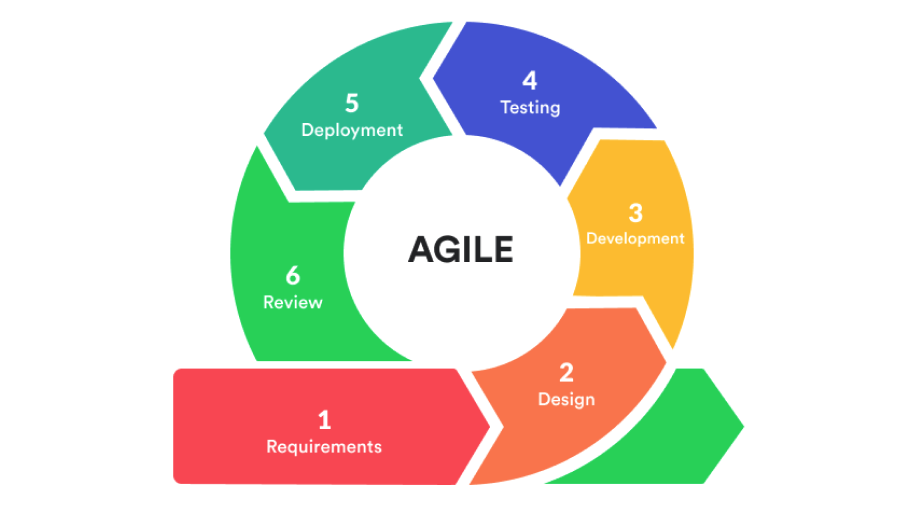
\includegraphics[width=0.8\textwidth]{images/agile-cycle.png}
    \caption{Agile Software Development Lifecycle}
    \label{fig:agile-cycle}
\end{figure}

A Agile Software Development Lifecycle iteration consists of several key stages like in Figure starting with planning phase where requirements for the iterartion are gathered and pritorized.

Since agile focuses adaptivity arising bugs can alter iterations if priotirised and therefore slow down delivery of features. APR is supposed to help with this problem by accelerating the process of fixing bugs.

Software development is moving towards lightly coupled microsversives which results in more repositories which are smaller in scale tailored towards a specialzed domain. This trend is driven by the need for flexibility, scalability, and faster development cycles. Smaller code repositories allow teams to work on specific components or services independently, reducing dependencies and enabling quicker iterations. This approach aligns with modern software development practices, such as microservices architecture and agile methodologies.
With this trend developers work on multiple projects at the same time, which can lead to more interrupptions and context swtiching when problems arise and priorities shift.



\subsection{Continuous Integration}

For accelerating the delviery of software in an iteration continous integration has become a standard in agile software development. 
Continuous Integration (CI) allows for frequenct code integration into a code repository. Ci often integrates automated building and testing giving rapid feedback right where the changes are made on the hosted repository.


Problems can be long build durations and high maintance \cite{ugwuezeContinuousIntegrationDeployment2024}

CI supports aspects like fast delivery, fast feedback, enhanced collaboration which are ciritcal for agile software development. 

\subsection{project hosting platforms}
Most software projects are hosted on platform like Github. But github is more than just a storage for repositories. It provides tools and feature for the complete software development lifecycle. Project hosting, verssion control, bug and issue tracking, project management, backups, collaboration, and documentation. \cite{abrahamssonAgileSoftwareDevelopment2017}




github is whre open soruces lives and development takes place. It is a platform that allows developers to host, share, and collaborate on code repositories. GitHub provides version control, issue tracking, and collaboration tools, making it a popular choice for open-source projects and software development teams.

allows for integration of systems like rennovate


\section{LLMs in Software Engineering}

modern large language models have billions of paramters, are pre-tained on massive codesbases which results in extraordinary capbilites in this area  \cite{chenUnveilingPitfallsUnderstanding2025}.

% TODO cite 
problems with llms are: Information leakage, hallucinations, and security issues

first LLms now research is looking into developing and improving workflows leveraging LLMs \cite{puvvadiCodingAgentsComprehensive2025}.

% TODO cite 
problems wi
looking into Agents using tools, LLMs + RAG,

\section{Automated Programm Repair}

Automated Program Repair (APR) helps developers fix bugs

localization, repair, and validation


\subsection{Evolution of Automated Program Repair}
% TODO cite 
Earliest APR techniques were based on version control history, using the history to roll back to a previous version of the code part, where no issues were present. This approach, while effective in some cases, often lacked the ability to perserve new features. (more like instant rollback)
history based

--- search based repair,

---semantic based repair,

---tempalte based repair,
apply predefined transformtions to the code based on rules

---The emerge of llm based techniques
LLM based APR techniques have demonstrated siognificant uimrpovemetns over all other state of the art technqiues, benfitintting from theor coding knowledge \cite{hossainDeepDiveLarge2024}

Agent Based
agent based system improve fixing abilites by probiding llms the ability to interact with the code base and the environment, allowing them to plan their actions  \cite{yangSWEagentAgentComputerInterfaces2024}.

llms lay the groundwork of a new APR paradigm \cite{chenUnveilingPitfallsUnderstanding2025}

complex agent arcitectures produce good results espically paired with containerized environments. Emphasis on quality insureance and Devops practices \cite{puvvadiCodingAgentsComprehensive2025}


modern aprs usally consist of multiple stages, including localization, repair, and validation. These stages are often implemented as separate modules, allowing for flexibility and modularity in the repair process \cite{yangSWEagentAgentComputerInterfaces2024}.

\subsection{Related Work - Existing Systems}


end to end without llms Sapfix from Facebook. Fixing bugs in production envrioments lowerring incidents mean time of recovery significantly \cite{margineanSapFixAutomatedEndtoEnd2019}

FixAgent \cite{leeUnifiedDebuggingApproach2024}

swe agent \cite{yangSWEagentAgentComputerInterfaces2024}

Agentless minimal system \cite{xiaAgentlessDemystifyingLLMbased2024}
claims exsiting systems are too complex and compute/costs intensive.
lacks the ability to control the decision planning.
they use a minimalist approach using localization, repair and validation.


this appraoch inspried the thesis to test how a simple approach will perform in a real world scendario on a code hosting platform.


--point out areas where current systems see limitation

-- during the research for this thesis, full integrations where published by companies like OpenAI Codex and Github Copilot - but these are not open source


\subsection{APR in CI Context}

CI allows seemless integration...
this way there is no harmfull code executed on own machiene, its encapsulated mutliple times container in Ci runner


\chapter{Methodology}
[Beschreibung des geplanten Vorgehens(-modells) zur L\"osung der Problemstellung; umfasst u.a.:
\begin{itemize}
  \item Anforderungserhebung und -analyse
  \item Konzeption, Entwurf
  \item Umsetzung (Implementierung)]
\end{itemize}

\section{Ergebnisartefakte}
 [Beschreibung der Ergebnisse / Ergebnistypen, welche Sie im Rahmen der Probleml\"osung generieren / erzielen wollen, z.B. Algorithmus, Prototyp einer Software(komponente), ... ]

\section{Datenschutzaspekte}
 [Beschreibung von Aspekten des Datenschutzes im Zusammenhang mit Ihrer Abschlussarbeit]

\section{Ethische Aspekte}
 [Beschreibung von Aspekten der Ethik\footnote{vgl. hierzu erg\"anzend allgemeine Codizes (z.B. \autocite{acm}, \autocite{ieee} oder \autocite{gi}) sowie auch domain-spezifische Normen und Verfahrensweisen im Rahmen einer kritischen Reflektion.}im Zusammenhang mit Ihrer Abschlussarbeit]


\chapter{Implementation}

[Beschreibung der Implementierung\footnotemark auf Basis des Entwurfs und der Methodologie / der geplanten Vorgehensweise zur Probleml\"osung im Kontext der Anforderungen. Hier ist Raum f\"ur Listings, wie z.B. das nun Folgende:


\footnotetext{Beachten Sie bei der Implementierung und deren Dokumentation bitte Clean Code Empfehlungen (vgl. hierzu z.B. \autocite{martin2008}).}

\begin{lstlisting}[caption={Ein Beispiel: Hello World (Scala)}]
object HelloWorld {
def main(args: Array[String]): Unit = {
  println("Hello, world!")
}
}
\end{lstlisting}

Umfangreicher Quell-Code sollte in den Anhang ausgelagert werden.]


\chapter{Results}

[Beschreibung der Ergebnisse aus allen voran gegangenen Kapiteln sowie der zuvor generierten Ergebnisartefakte mit Bewertung, wie diese einzuordnen sind]


\chapter{Discussion}
\input{chapter/06-discussion.tex}

\chapter{Conclusion}
[Aggregierte retrograde Kurzbeschreibung der Arbeit]
\section{Schlussfolgerungen}
 [Beschreibung der insgesamt zu konstatierenden Schlussfolgerungen im Zusammenhang mit der Arbeit]
\section{Limitationen}
 [Beschreibung der Ergebnisse einer kritischen Reflektion und Begr\"undung dessen, was die Arbeit nicht zu leisten vermag]
\section{Ausblick}
 [Beschreibung und Begr\"undung potenzieller zuk\"unftiger Folgeaktivit\"aten im Zusammenhang mit Ihrer Arbeit (z.B. weitere Anforderungen, Theoriebildung, ... ]


%----------------------------------------------------------------------------------------
%	REFERENCE LIST
%----------------------------------------------------------------------------------------

\printbibliography[
  heading=bibintoc,
  title={References}
]



\newpage

\chapter{Abk\"urzungsverzeichnis}

\newpage

\chapter{Glossar}

\appendix

\chapter{Appendix} \label{chapter:appendix}

\section{Source Code and Data}
The source code of the thesis is available on GitHub split in two repositories. Both repositories have Readme files that explain how to use the code and data. 
\begin{itemize}
    \item \textbf{Prototype Repository:} Contains the implementation of the APR Core and the CI configuration. It is available at: \url{https://github.com/justingebert/bugfix-ci}
    \item \textbf{Evaluation Repository:} Contains the evaluation scripts and results of the APR system, including the QuixBugs benchmark setup. It is available at: \url{https://github.com/justingebert/quixbugs-apr}
\end{itemize}


\section{LLM Versions}
The following Table lists the exact LLM versions that where used during development and evaluation. 
\begin{longtable}{p{5cm} | p{6cm}}
    \caption{LLM models and their versions used in the system} \label{table:llm_versions} \\
    \hline
    \textbf{Model Name} & \textbf{Version} \\
    \hline
    \endfirsthead
    \hline
    \endfoot
    gemini-2.0-flash-lite    & gemini-2.0-flash-lite \\
    gemini-2.0-flash         & gemini-2.0-flash \\
    gemini-2.5-flash-lite & gemini-2.5-flash-lite-preview-06-17 \\
    gemini-2.5-flash         &  gemini-2.5-flash\\
    gemini-2.5-pro           & gemini-2.5-pro \\
    gpt-4.1-nano             & gpt-4.1-nano-2025-04-14 \\
    gpt-4.1-mini             & gpt-4.1-mini-2025-04-14 \\
    gpt-4.1                  & gpt-4.1-2025-04-14 \\
    o4-mini                  & o4-mini-2025-04-16 \\
    claude-3-5-haiku         & claude-3-5-haiku-20241022 \\
    claude-3-7-sonnet        & claude-3-7-sonnet-20250219 \\
    claude-sonnet-4-0        & claude-sonnet-4-20250514 \\
    \hline
\end{longtable}

\newpage

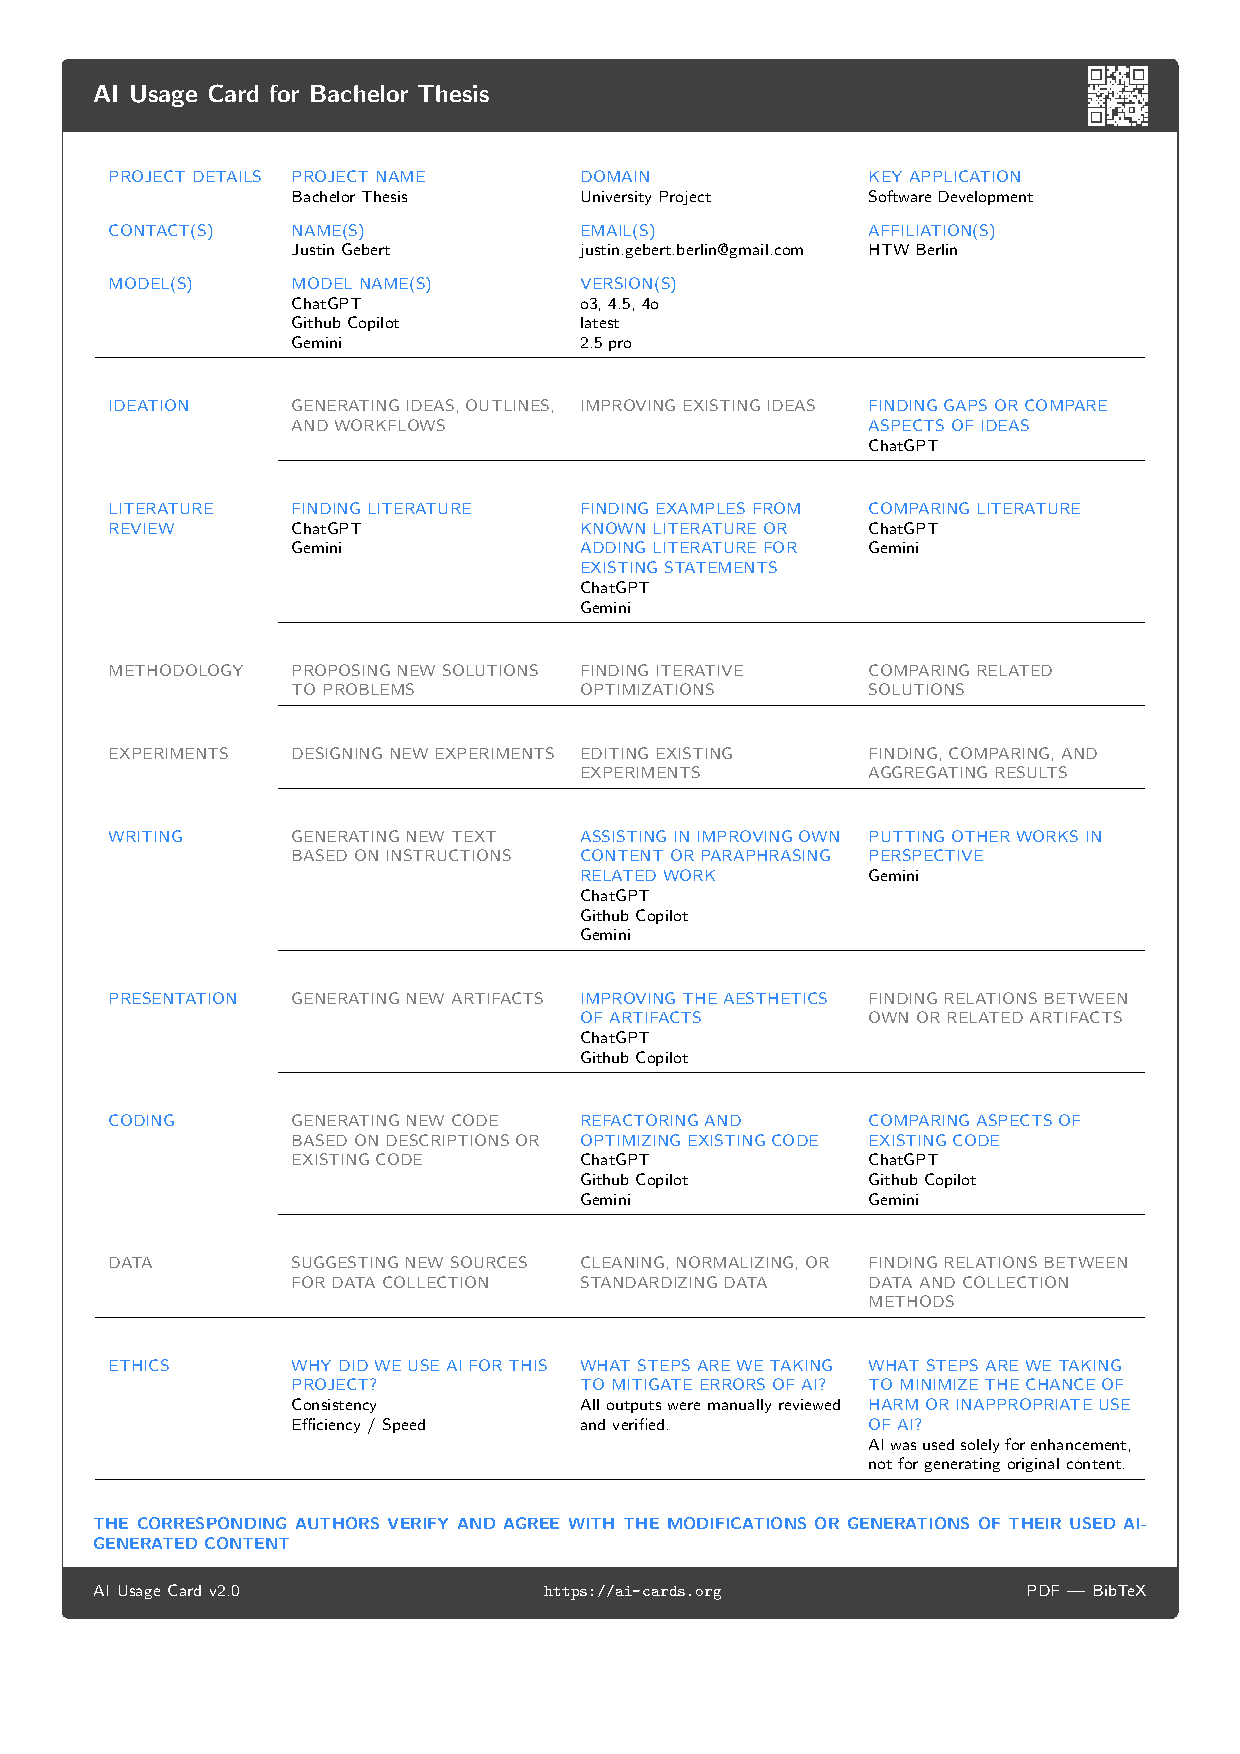
\includepdf[pages={1}]{pages/Ai-usage-card.pdf}

\thispagestyle{empty}
%\vspace*{18cm}
\noindent


\section*{Eidesstattliche Versicherung}
Hiermit versichere ich an Eides statt durch meine Unterschrift, dass ich die vorstehende Arbeit selbstst\"andig und ohne fremde Hilfe angefertigt und alle Stellen, die ich w\"ortlich oder ann\"ahernd w\"ortlich aus Ver\"offentlichungen entnommen habe, als solche kenntlich gemacht habe, mich auch keiner anderen als der angegebenen Literatur oder sonstiger Hilfsmittel bedient habe. Die Arbeit hat in dieser oder \"ahnlicher Form noch keiner anderen Pr\"ufungsbeh\"orde vorgelegen.\\
\linebreak[4]
\linebreak[4]
\linebreak[4]
\linebreak[4]
-------------------------------------------------------\linebreak[4]
Datum, Ort, Unterschrift

\end{document}